\chapter{Release 2}


\section{Introduction}

Dans ce chapitre, il s'agit d'un release qui consiste en un seul sprint qui est la consultation des rapports ,
afin de pouvoir repr\'{e}senter ces rapports ,nous avons besoins d'abord de determiner
les axes de notre \'{e}tude d\'{e}cisonnelle , puis nous allons \'{e}laborer et tester les rapports en utilisant l'outil Power BI
ensuite nous illustrons la partie ETL(Extract Trasform Load) \`{a} l'aide du l'outil Talend,
et nous finissons par la pr\'{e}sentation des rapports obtenues.

\section{ Analyse et conception}
\subsection{Analyse}


\subsubsection{ Diagramme de cas d'utilisation "Consultation des rapports"}

\begin{figure}[H]
\center
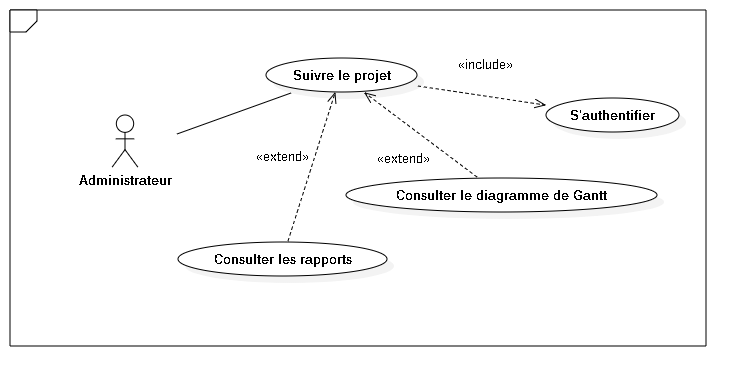
\includegraphics[width=13cm,height=8cm]{./figures/ucS.png}
\caption{G\'{e}rer un projet.}

\end{figure}

\subsection{Conception}

\subsubsection{Le sc\'{e}nario \guillemotleft{} Consultation des rapports\guillemotright{}}
Le diagramme de s\'{e}quence \guillemotleft{} Ajout d'une t\^{a}che \guillemotright{} pr\'{e}sente le s\'{e}quencement
des interactions entre Administrateur, Application et Base de donn\'{e}es (BD).


\begin{figure}[H]
\center
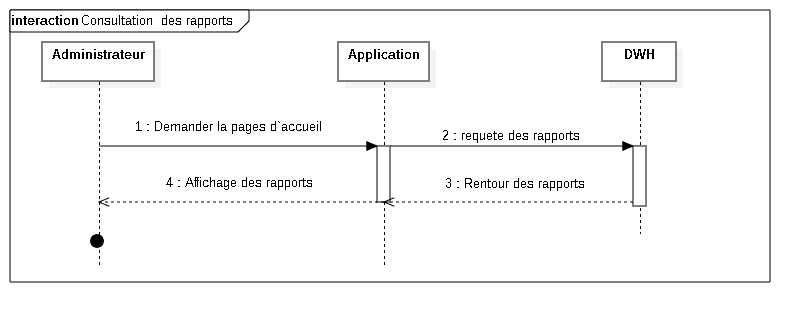
\includegraphics[width=14cm,height=9cm]{./figures/seq/G.png}
\caption{Consultation des rapports.}
\end{figure}


\section{ But de l'\'{e}tude d\'{e}cisionnelle }

Notre \'{e}tude d\'{e}cisionnelle portera sur :

\textbullet{} Le co\^{u}t total de chaque projet
\textbullet{} Le co\^{u}t total des projets pour chaque client
\textbullet{} Le co\^{u}t total par cat\'{e}gorie des projets
\textbullet{} La dur\'{e}e totale du chaque projet
\bigskip
\section{ Elaboration des rapports sur Power BI }
\subsubsection{Pr\'{e}paration}
Nous avons besoin d'ajuster quelques champs pour \^{e}tre ad\'{e}quates \`{a} \^{e}tre
exploit\'{e}es . Par exemple dans la table membre on trouve " firstname " et
"lastname" Et on doit les concat\'{e}ner pour dans une hi\'{e}rarchie pour avoir
des rapports lisibles \`{a} propos des membres .




\FloatBarrier
\begin{figure}[H]
\center
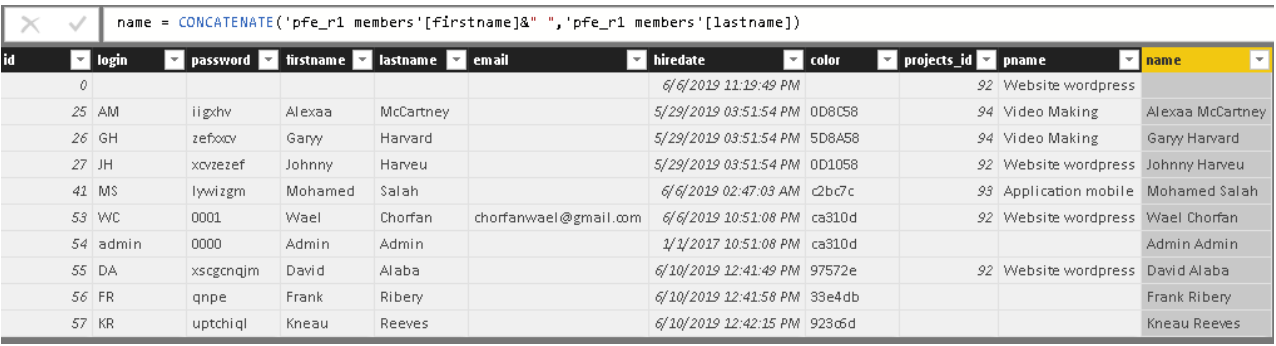
\includegraphics[width=14cm,height=5cm]{./figures/pb1.png}
\caption{Ajustement des noms.}
\end{figure}
\FloatBarrier


\bigskip
\bigskip

\FloatBarrier
\begin{figure}[H]
\center
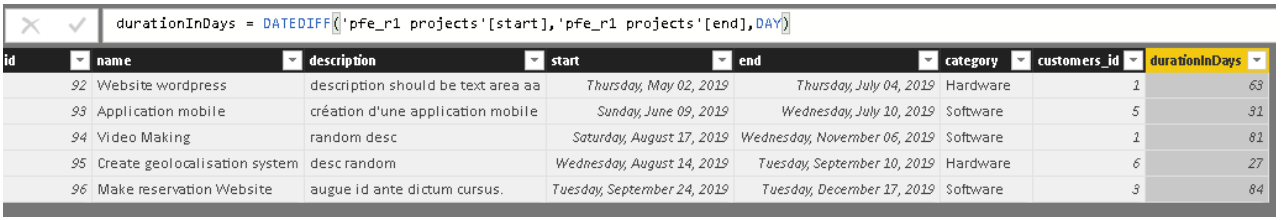
\includegraphics[width=14cm,height=3cm]{./figures/pb2.png}
\caption{Ajustement de la dur\'{e}e totale des projets.}
\end{figure}
\FloatBarrier

\newpage
\subsubsection{Reporting  sur Power BI}
Pour tester les rapports et la validit\'{e} des donn\'{e}es , nous avons utilis\'{e} l'outil
Power BI pour nous donner une impression sur les rapports qu'on doit
int\'{e}grer \`{a} notre application afin de les visulaiser.

\bigskip
Pour ce fait on a cr\'{e}e les rapports correspontdants \`{a} l'\'{e}tude d\'{e}cisionnelle :
Les deux axes importants de l'\'{e}tude sont les couts et la dur\'{e}e :



\begin{itemize}

\item{ \textbf{Les  co\^{u}ts}  }

\FloatBarrier
\begin{figure}[H]
\center
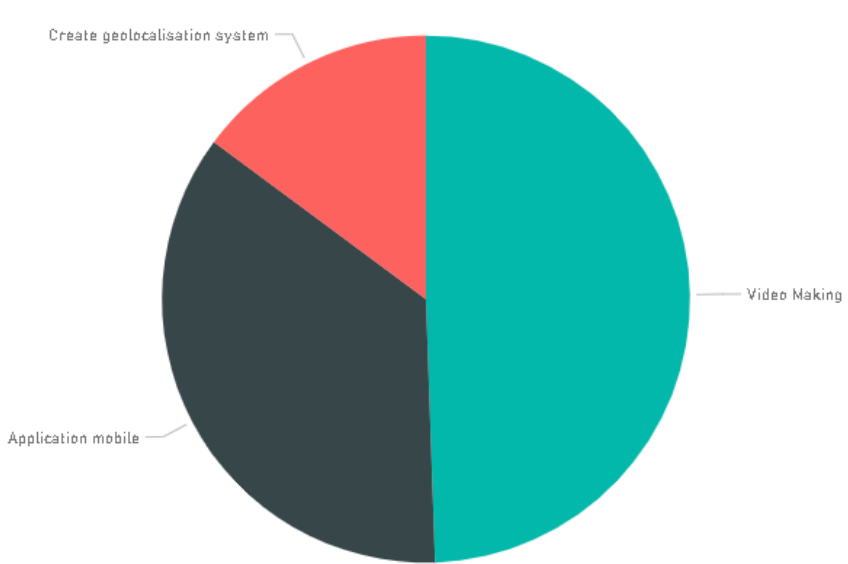
\includegraphics[width=10cm,height=10cm]{./figures/rpb1.png}
\caption{Co\^{u}t total par projet.}

\end{figure}
\FloatBarrier

\FloatBarrier
\begin{figure}[H]
\center
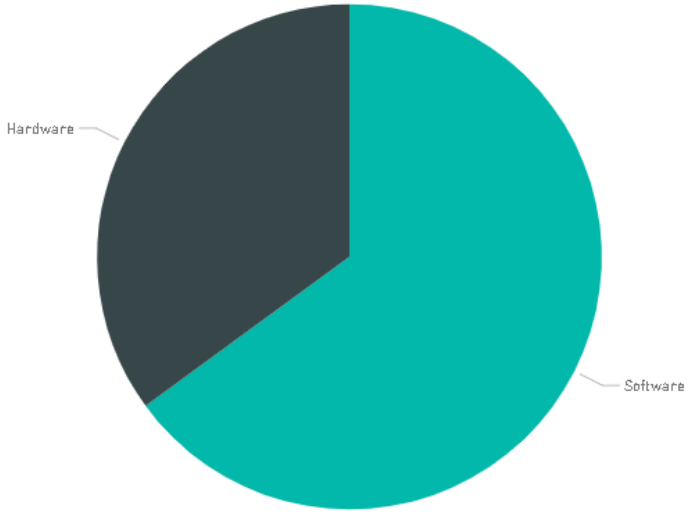
\includegraphics[width=10cm,height=10cm]{./figures/rpb2.png}
\caption{Co\^{u}t total par catégorie de projet.}

\end{figure}
\FloatBarrier

\FloatBarrier
\begin{figure}[H]
\center
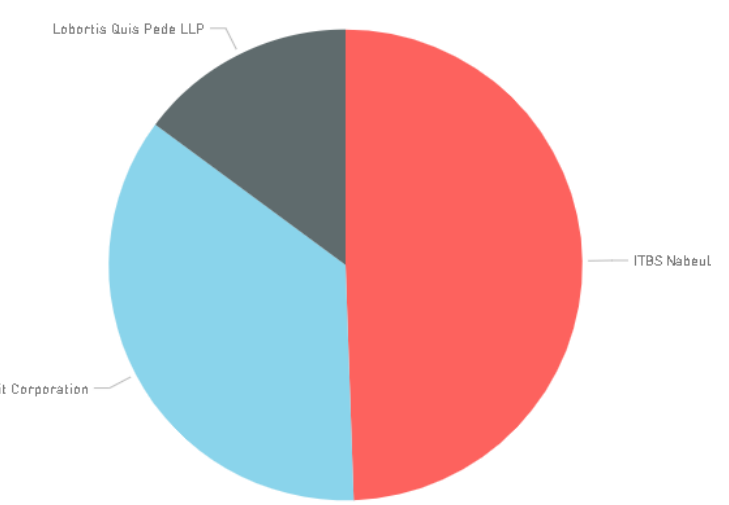
\includegraphics[width=10cm,height=10cm]{./figures/rpb3.png}
\caption{Co\^{u}t total par client.}

\end{figure}
\FloatBarrier

\FloatBarrier
\begin{figure}[H]
\center
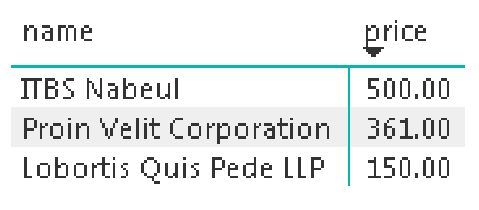
\includegraphics[width=8cm,height=5cm]{./figures/rpb31.png}
\caption{Co\^{u}t total par client en chiffres.}

\end{figure}
\FloatBarrier



\newpage

\item{ \textbf{La dur\'{e}e}  }
\FloatBarrier
\begin{figure}[H]
\center
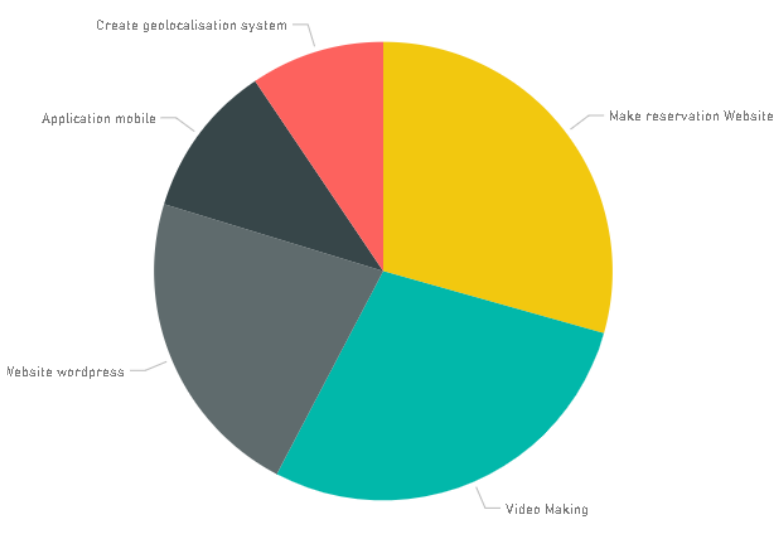
\includegraphics[width=10cm,height=10cm]{./figures/rpb4.png}
\caption{Dur\'{e}e total par projet (en jours).1}

\end{figure}
\FloatBarrier

\FloatBarrier
\begin{figure}[H]
\center
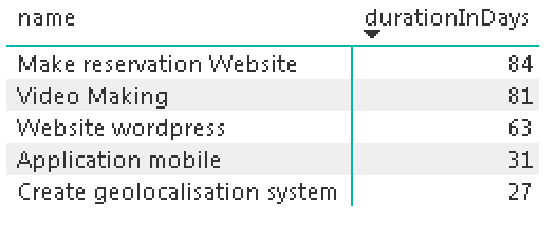
\includegraphics[width=8cm,height=5cm]{./figures/rpb42.png}
\caption{Dur\'{e}e total par projet (en jours).2}

\end{figure}
\FloatBarrier


\end{itemize}




















































\section{ Partie ETL }
Pour avoir des rapports sur l'application web ,on doit avoir les donn\'{e}es sous une certaine format ,
afin de satisfaire le besoin de la consultation du suivi des projets selon le temps et le cout.
Ains les donn\'{e}es correspondantes sont collect\'{e}es, modifi\'{e}es et charg\'{e}es dans un entrep\^{o}t de donn\'{e}es
assurant ainsi la phase ETL.

Nous avons utilis\'{e} l'outil talend pour charger les donn\'{e}es n\'{e}cessaires .
Puisque nous avons les donn\'{e}es ordonn\'{e}es et int\'{e}gres ,nous n'avons pas \'{e}t\'{e} besoin d'une ODS (Operational data source)
nous passont directement \`{a} construite notre table de faits



\subsection{Int\'{e}gration}


Pour obtenir les co\^{u}ts nous avons calcul\'{e} le prix par chaque projet 
,cat\'{e}gorie ,et nom du client.

\begin{figure}[H]
\center
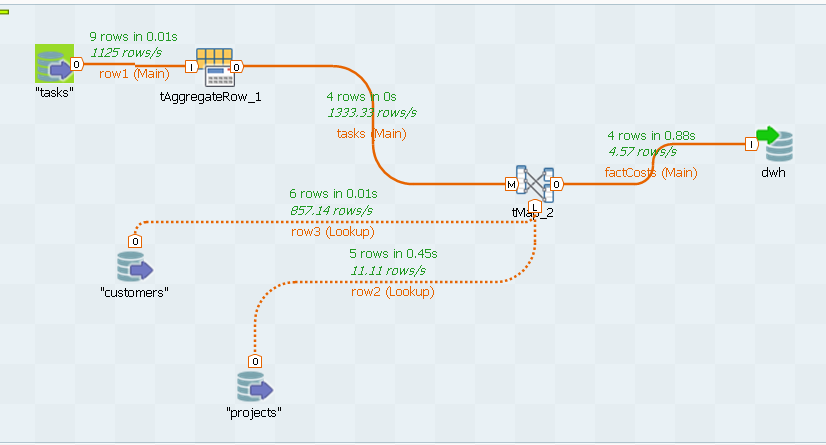
\includegraphics[width=14cm,height=9cm]{./figures/integ.png}
\caption{Extraction des co\^{u}ts.1.}
\end{figure}



\begin{figure}[H]
\center
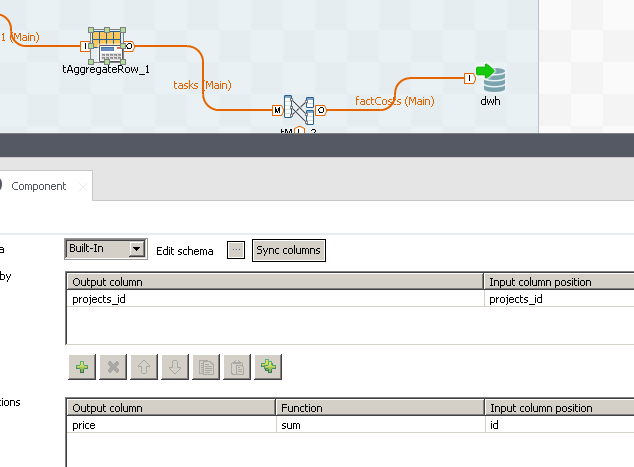
\includegraphics[width=14cm,height=9cm]{./figures/integ1.png}
\caption{Extraction des co\^{u}ts.2.}
\end{figure}


\begin{figure}[H]
\center
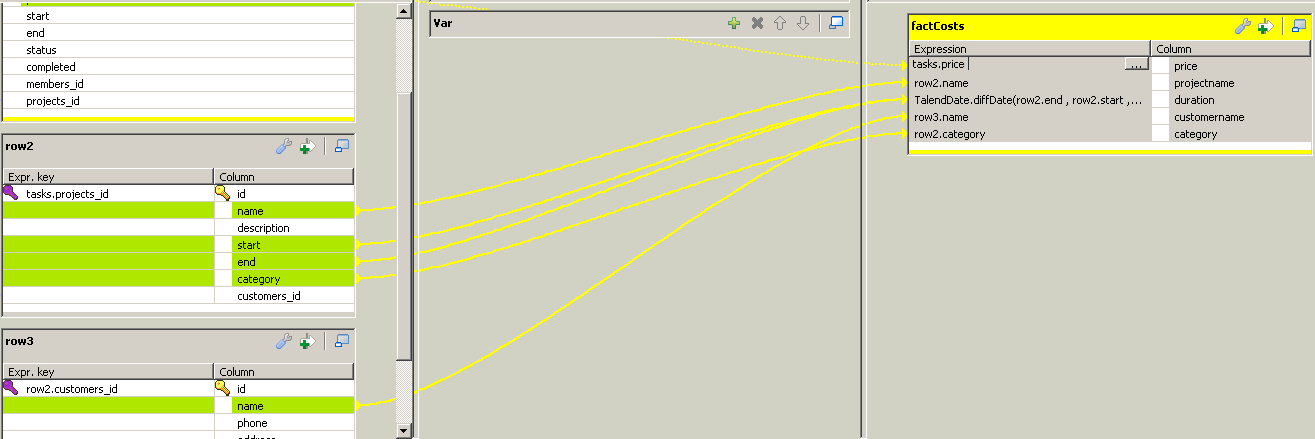
\includegraphics[width=14cm,height=9cm]{./figures/integ3.png}
\caption{Extraction des co\^{u}ts.3.}
\end{figure}



Pour obtenir la dur\'{e}e du chaque projet en jours ,
nous avons calcul\'{e} pour chaque projet la diff\'{e}rence en jours .

\begin{figure}[H]
\center
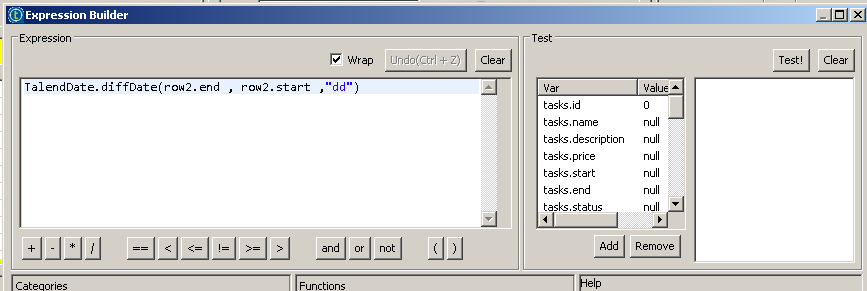
\includegraphics[width=14cm,height=9cm]{./figures/integ2.png}
\caption{Extraction des  dur\'{e}es.}
\end{figure}



\subsection{Sh\'{e}mas obtenus}
A partir du du sh\'{e}ma de la fig \`{a} on a obtenue la table fact selon ce shéma
\FloatBarrier

\begin{figure}[H]
\center
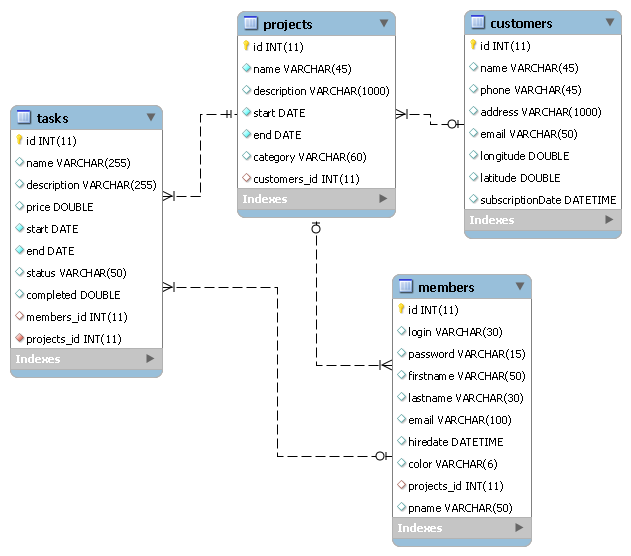
\includegraphics[width=14cm,height=9cm]{./figures/s1.png}
\caption{Sh\'{e}ma initial.}
\end{figure}
\FloatBarrier


\FloatBarrier

\begin{table}
\centering
\begin{tabular}{|l|l|l|l|l|l|l|}
\hline
Field        & Type         & Null & Key & Default & Extra &   \\
\hline
price        & double(22,0) & YES  &     & NULL    &       &   \\
\hline
projectname  & varchar(45)  & NO   &     & NULL    &       &   \\
\hline
duration     & bigint(10)   & NO   &     & NULL    &       &   \\
\hline
customername & varchar(45)  & YES  &     & NULL    &       &   \\
\hline
category     & varchar(60)  & YES  &     & NULL    &       &   \\
\hline
\end{tabular}
\end{table}
\FloatBarrier


les donn\'{e}es obtenues sont comme suit :
\begin{table}
\centering
\begin{tabular}{|l|l|l|l|l|}
\hline
price & projectname                   & duration & customername            & category  \\
\hline
66    & Website wordpress             & 63       & ITBS Nabeul             & Hardware  \\
\hline
121   & Application mobile            & 31       & Proin Velit Corporation & Software  \\
\hline
81    & Video Making                  & 81       & ITBS Nabeul             & Software  \\
\hline
43    & Create geolocalisation system & 27       & Lobortis Quis Pede LLP  & Hardware  \\
\hline
\end{tabular}
\end{table}
\FloatBarrier




\subsubsection{Test}

Si l'administrateur parvient \`{a} ese connecter il trouve cette interface d'accueil
ou il trouvera les rapports qui d\'{e}crivent des statistiques primordiales au
d\'{e}oulement des projets donc les interfaces et les fonctionnalit\'{e}s disponibles
pour l'admin sont :

\subsection{La consultation des rapports}


\FloatBarrier
\begin{figure}[H]
\center
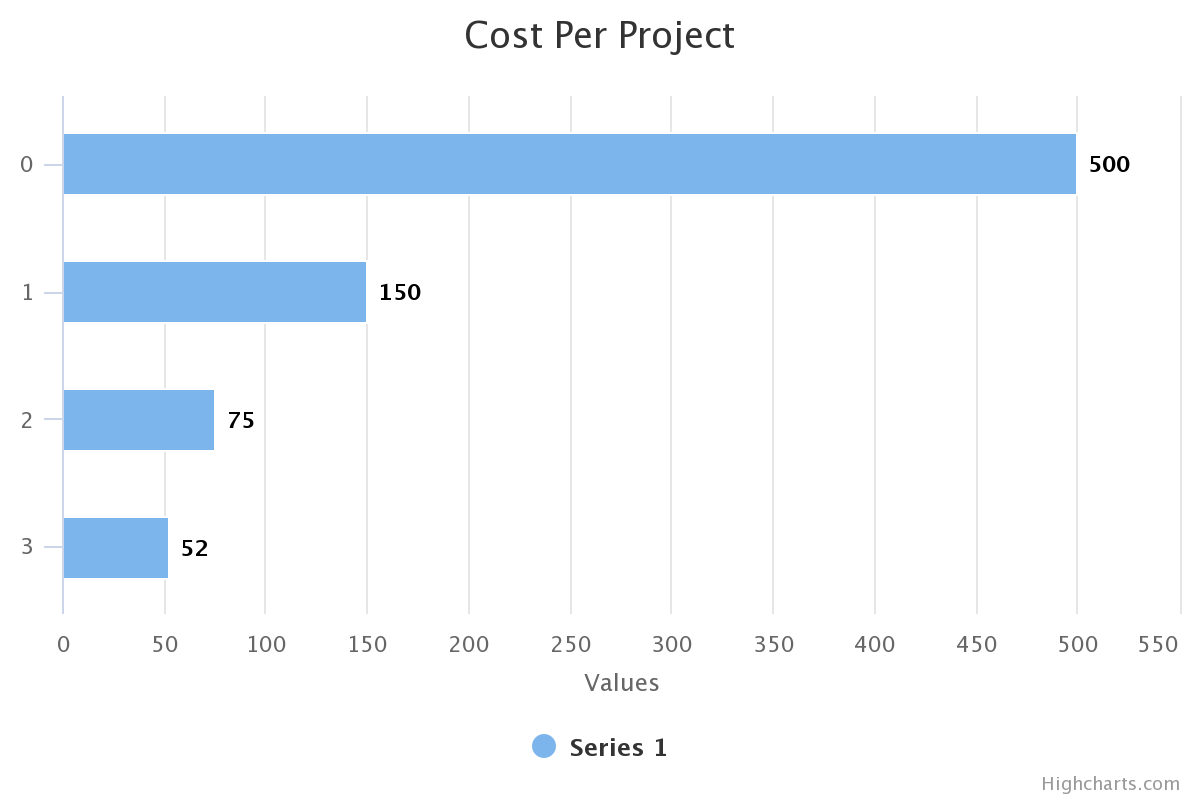
\includegraphics[width=11cm,height=7cm]{./figures/pres/cost-per-project.png}
\caption{ Co\^{u}t par projet }
\end{figure}
\FloatBarrier

\FloatBarrier
\begin{figure}[H]
\center
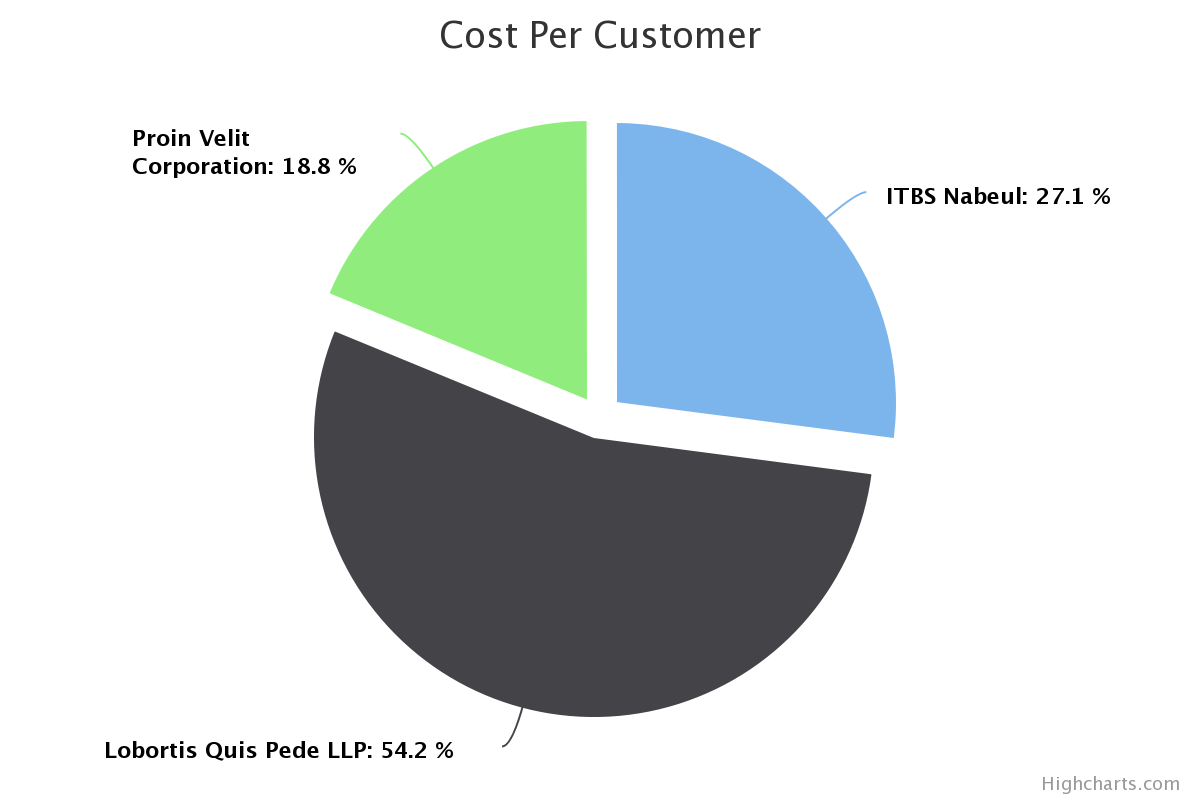
\includegraphics[width=11cm,height=7cm]{./figures/pres/cost-per-customer.png}
\caption{ Co\^{u}t par client }
\end{figure}
\FloatBarrier

\FloatBarrier
\begin{figure}[H]
\center
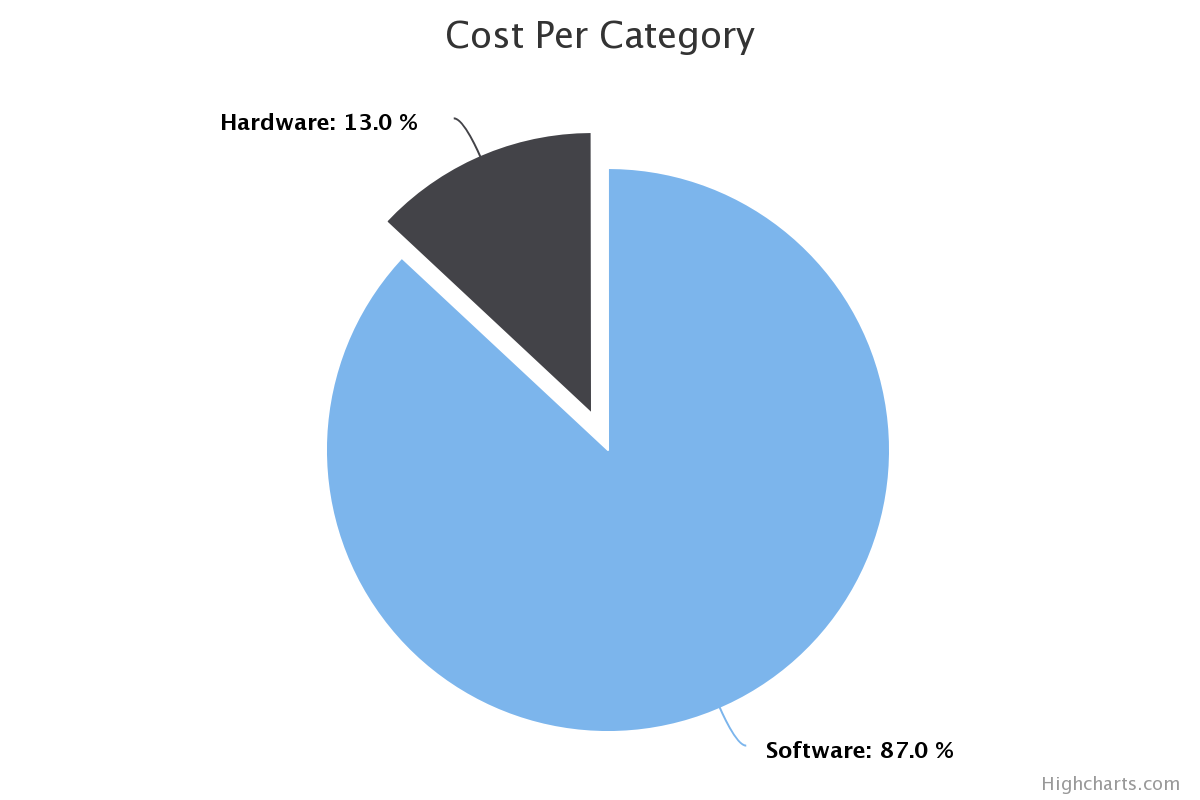
\includegraphics[width=11cm,height=7cm]{./figures/pres/cost-per-category.png}
\caption{ Co\^{u}t par cat\'{e}gorie}
\end{figure}
\FloatBarrier

\FloatBarrier
\begin{figure}[H]
\center
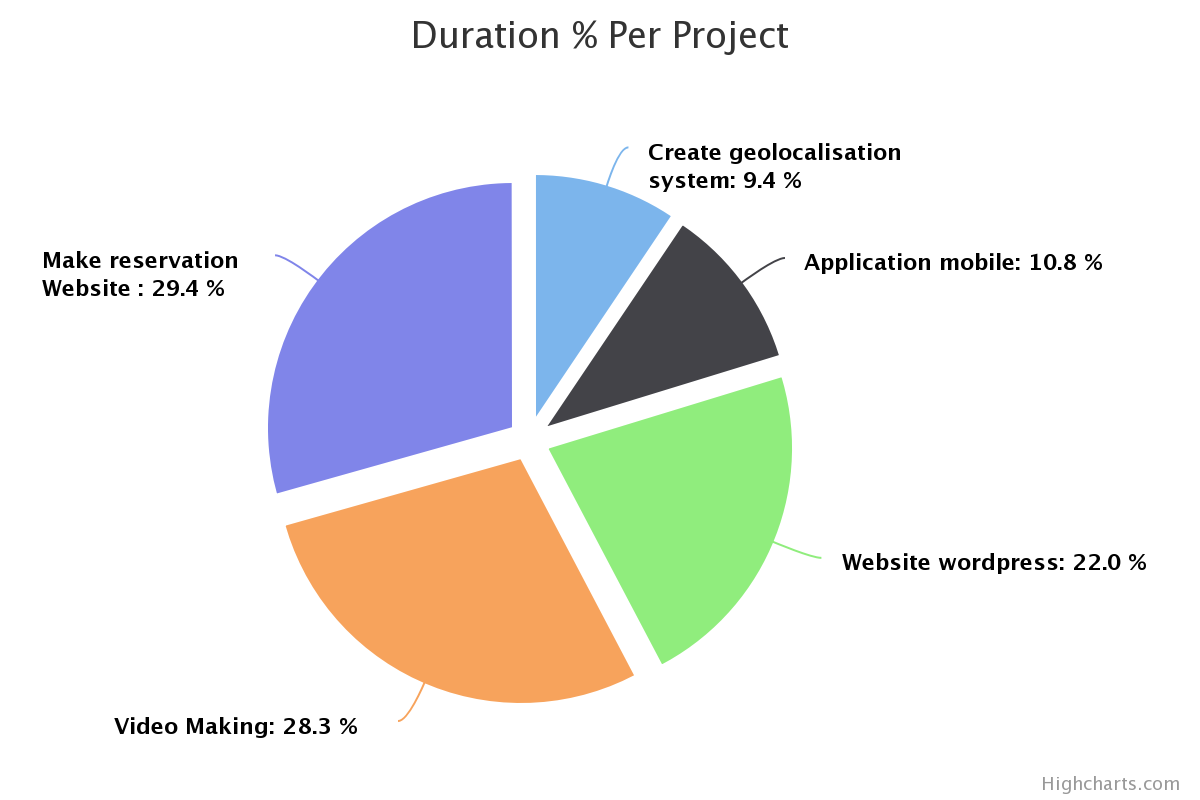
\includegraphics[width=11cm,height=7cm]{./figures/pres/duration-per-project.png}
\caption{Dur\'{e}e par projet.1. }
\end{figure}
\FloatBarrier

\FloatBarrier
\begin{figure}[H]
\center
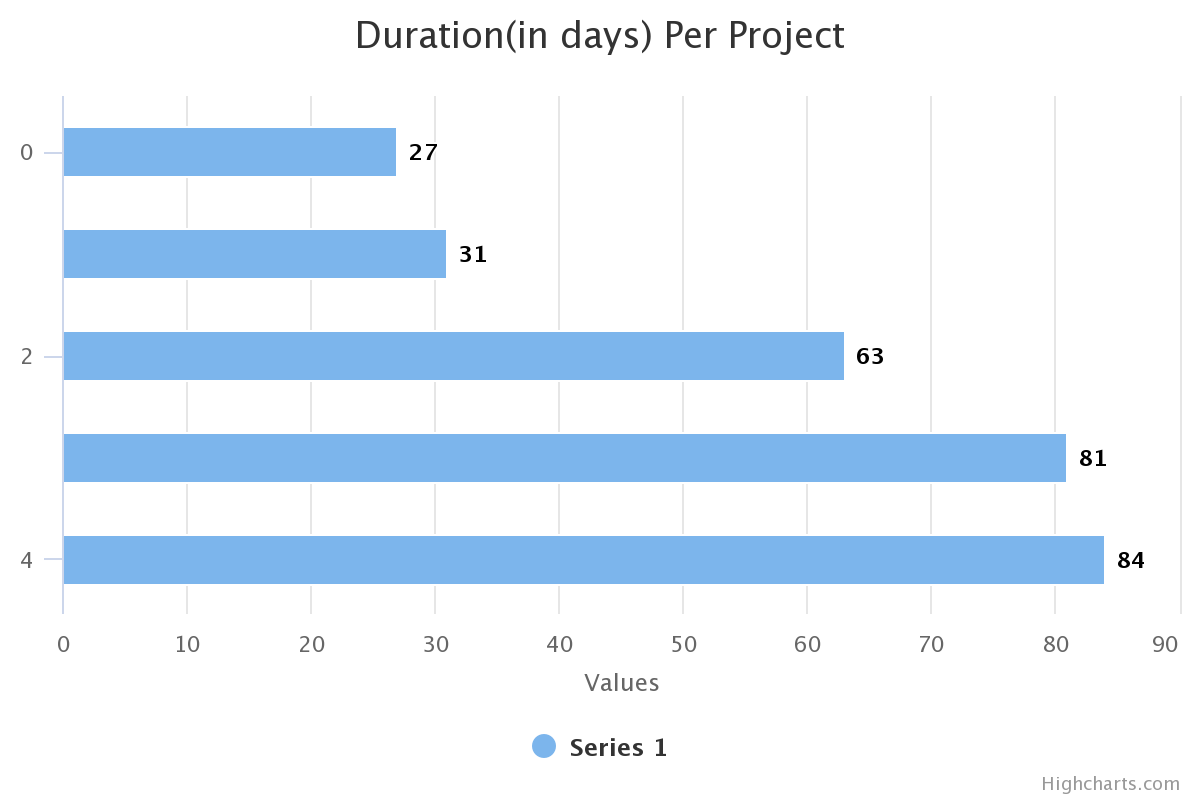
\includegraphics[width=11cm,height=7cm]{./figures/pres/durationin-days-per-proj.png}
\caption{Dur\'{e}e par projet.2.}
\end{figure}
\FloatBarrier









